\section{Single Page Application: Pros and Cons}
\label{sec:ARC_overview}

One benefit of SPAs is obvious: Applications are more fluid and responsive, without the jarring effect of reloading and re-rendering the page. Another benefit might be less obvious and it concerns how you architect a Web app. Sending the app data as JSON creates a separation between the presentation (HTML markup) and application logic (AJAX requests plus JSON responses).
This separation makes it easier to design and evolve each layer. In a well-architected SPA, you can change the HTML markup without touching the code that implements the application logic (at least, that’s the ideal). You’ll see this in action when I discuss data binding later.
In a pure SPA, all UI interaction occurs on the client side, through JavaScript and CSS. After the initial page load, the server acts purely as a service layer. The client just needs to know what HTTP requests to send. It doesn’t care how the server implements things on the back end.
With this architecture, the client and the service are independent. You could replace the entire back end that runs the service, and as long as you don’t change the API, you won’t break the client. The reverse is also true—you can replace the entire client app without changing the service layer. For example, you might write a native mobile client that consumes the service. NOTA 3

\begin {figure}[h]
\graphicspath{{images/chapter_arc/}}
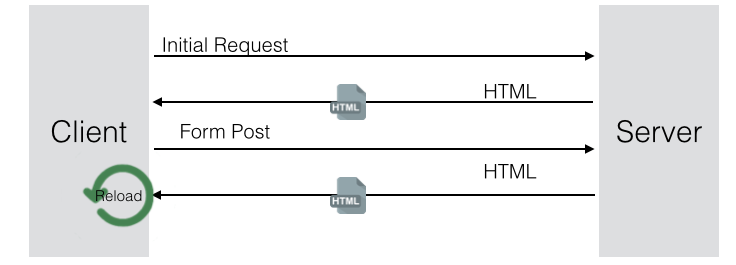
\includegraphics[width=\textwidth]{trad_life}
\caption{The Traditional Page Lifecycle}
\end {figure}


\begin {figure}[h]
\graphicspath{{images/chapter_arc/}}
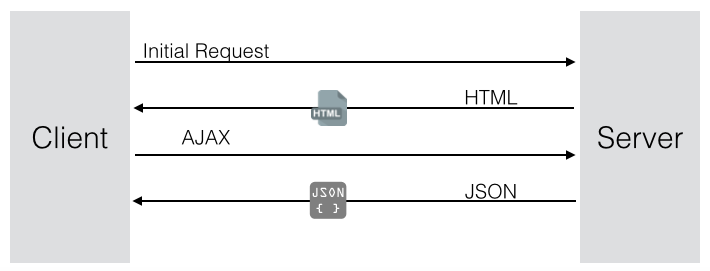
\includegraphics[width=\textwidth]{spa_life}
\caption{The SPA Lifecycle}
\end {figure}



Because the SPA is an evolution away from the stateless page-redraw model that browsers were originally designed for, some new challenges have emerged. Each of these problems has an effective solution with:
\begin{itemize}
\item Client-side JavaScript libraries addressing various issues.
\item Server-side web frameworks that specialize in the SPA model.
\item The evolution of browsers and the HTML5 specification aimed at the SPA model.
\end{itemize}

\subsection{Search engine optimization (SEO)}
\label{subsec:arc_over_seo}
Because of the lack of JavaScript execution on crawlers of some popular Web search engines, SEO (Search engine optimization) has historically presented a problem for public facing websites wishing to adopt the SPA model.
Google currently crawls URLs containing hash fragments starting with \#!. This allows the use of hash fragments within the single URL of an SPA. Special behavior must be implemented by the SPA site to allow extraction of relevant metadata by the search engine's crawler. For search engines that do not support this URL hash scheme, the hashed URLs of the SPA remain invisible.
Alternatively, applications may render the first page load on the server and subsequent page updates on the client. This is traditionally difficult, because the rendering code might need to be written in a different language or framework on the server and in the client. Using logic-less templates, cross-compiling from one language to another, or using the same language on the server and the client may help to increase the amount of code that can be shared.
Because SEO compatibility is not trivial in SPAs, it's worth noting that SPAs are commonly not used in a context where search engine indexing is either a requirement, or desirable. Use cases include applications that surface private data hidden behind an authentication system. In the cases where these applications are consumer products, often a classic page redraw model is used for the applications landing page and marketing site, which provides enough meta data for the application to appear as a hit in a search engine query. Blogs, support forums, and other traditional page redraw artifacts often sit around the SPA that can seed search engines with relevant terms.
Another approach used by server-centric web frameworks like the Java-based ItsNat is to render any hypertext in the server using the same language and templating technology. In this approach, the server knows with precision the DOM state in the client, any big or small page update required is generated in the server, and transported by AJAX, the exact JavaScript code to bring the client page to the new state executing DOM methods. Developers can decide which page states must be crawlable by web spiders for SEO and be able to generate the required state in load time generating plain HTML instead of JavaScript. In case of the ItsNat framework, this is automatic because ItsNat keeps the client DOM tree in the server as a Java W3C DOM tree; rendering of this DOM tree in the server generates plain HTML in load time and JavaScript DOM actions for AJAX requests. This duality is very important for SEO because developers can build with the same Java code and pure HTML-based templating the desired DOM state in server; on page load time, conventional HTML is generated by ItsNat making this DOM state SEO-compatible. As of version 1.3, ItsNat provides a new stateless mode, client DOM is not kept in the server because, in stateless mode client, DOM state is partially or fully reconstructed in the server when processing any AJAX request based on required data sent by client informing of the current DOM state; the stateless mode may be also SEO-compatible because SEO compatibility happens in load time of the initial page not affected by stateful or stateless modes.
There are a couple of workarounds to make it look as though the web site is crawlable. Both involve creating separate HTML pages that mirror the content of the SPA. Server could create a HTML-based version of the site and deliver that to crawlers, or it's possible to use a headless browser such as PhantomJS to run JavaScript application and output the resulting HTML.
Both of these do require quite a bit of effort, and can end up giving a maintenance headache for the large complex sites. There are also potential SEO pitfalls. If server-generated HTML is deemed to be too different from the SPA content, then the site will be penalized. Running PhantomJS to output the HTML can slow down the response speed of the pages, which is something for which search engines – Google in particular – downgrades the rankings.


\subsection{Client/Server code partitioning}
\label{subsec:arc_over_code}
One way to increase the amount of code that can be shared between servers and clients is to use a logic-less template language like Mustache or Handlebars. Such templates can be rendered from different host languages, such as Ruby on the server and JavaScript in the client. However, merely sharing templates typically requires duplication of business logic used to choose the correct templates and populate them with data. Rendering from templates may have negative performance effects when only updating a small portion of the page—such as the value of a text input within a large template. Replacing an entire template might also disturb a user's selection or cursor position, where updating only the changed value might not. To avoid these problems, applications can use UI data bindings or granular DOM manipulation to only update the appropriate parts of the page instead of re-rendering entire templates. NOTA 2

\subsection{Analytics}
\label{subsec:arc_over_analytics}
Analytics tools such as Google Analytics rely heavily upon entire new pages loading in the browser, initiated by a URL change. SPAs don’t work this way.
After the first page load, all subsequent page and content changes are handled internally by the application. So the browser never triggers a new page load, nothing gets added to the browser history, and the analytics package has no idea who’s doing what on the site.

It's possible to add page load events to an SPA using the HTML5 history API; this will help integrate analytics. The difficulty comes in managing this and ensuring that everything is being tracked accurately – this involves checking for missing reports and double entries. Some frameworks provide open source analytics integrations addressing most of the major analytics providers. Developer should integrate them into the application and make sure that everything is working correctly, but there's no need to do everything from scratch.


\subsection{Speed of initial load}
\label{subsec:arc_over_speed}

Single Page Applications have a slower first page load than server-based applications. This is because the first load has to bring down the framework and the application code before rendering the required view as HTML in the browser. A server-based application just has to push out the required HTML to the browser, reducing the latency and download time.


There are some ways of speeding up the initial load of an SPA, such as a heavy approach to caching and lazy-loading modules when needed. But it's not possible to get away from the fact that it needs to download the framework, at least some of the application code, and will most likely hit an API for data before displaying something in the browser.This is a ``pay me now, or pay me later'' trade-off scenario. The question of performance and wait-times remains a decision that the developer must make.
NOTA 1

